\section{Motivation}
\label{sec:motivation}

% \todo{make sure we use queue(s) throughout the paper instead of user(s)}
%In this section, we demonstrate the benefits of temporal co-scheduling of queues with heterogeneous performance metrics using an example to compare against existing solutions (Section~\ref{sec:ex}). 
%Next, we explore the desired properties and the design space for such a solution (Section~\ref{sec:desire}), followed by the discussion of challenges in achieving high \burstq utilization by admitting more {\burstq}s with resource guarantee.
% Our model and solution approach apply to a general class of resource allocation problems including those in the networking community (Section~\ref{sec:networking}) \todo{add}.

%While hard guarantee and instantaneous fairness are with fundamental tradeoffs, (Section~\ref{sec:desire})  and.  and inefficiencies in existing schedulers (Section~\ref{sec:desire}), and discusses the challenges associated (Section~\ref{sec:challenge}).


\subsection{Benefits of Temporal Co-scheduling}
\label{sec:ex}


%\begin{figure}[!t]
%	\centering
%	
\includegraphics[width=0.3\linewidth]{fig/b1_mov_legend} 
%	\\
%	\subfloat[DRF: While instantaneous fairness is enforced, the completion time of \burstq jobs is much higher than that under SP.]{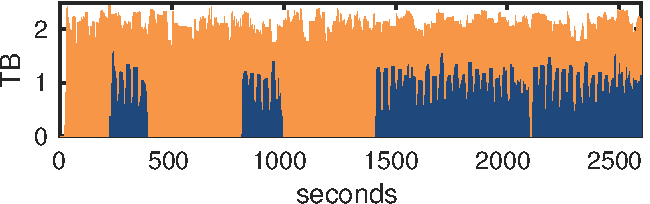
\includegraphics[width=0.8\linewidth]{fig/b1_mov_DRF_BB}\label{fig:motiv-DRF}}
%	%\subfloat[DRF -- The completion time of 4 \burstq jobs are  202, 178, 715, and 719 seconds, respectively.]{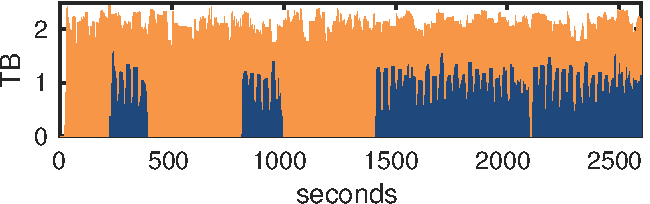
\includegraphics[width=1.0\linewidth]{fig/b1_mov_DRF_BB}\label{fig:motiv-DRF}}
%	\\
%	\subfloat[Strict Priority (SP): While the completion time of \burstq jobs are reduced, \batchq does not receive its fair share after \burstq increases its demand after 1,400 seconds.]{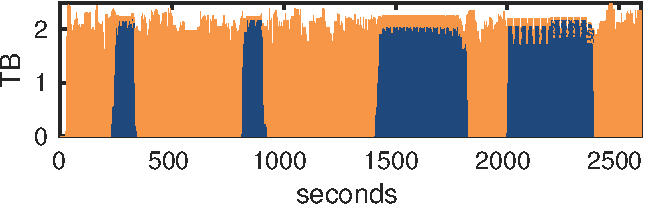
\includegraphics[width=0.8\linewidth]{fig/b1_mov_Strict_BB}\label{fig:motiv-Strict}}
%	%\subfloat[Strict Prority (SP)-- The completion time of 4 \burstq jobs are  124, 121, 430, and 405 seconds, respectively.]{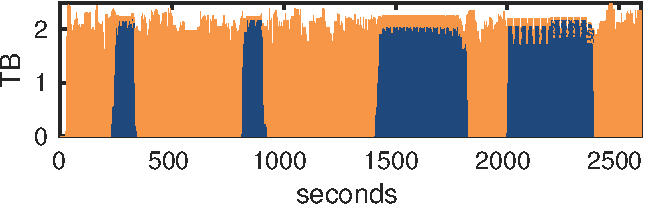
\includegraphics[width=1.0\linewidth]{fig/b1_mov_Strict_BB}\label{fig:motiv-Strict}	}
%	\\
%	\subfloat[Ideal: The first two \burstq jobs finish as quickly as possible. The latter jobs cannot use more resources than \burstq's fair share.]{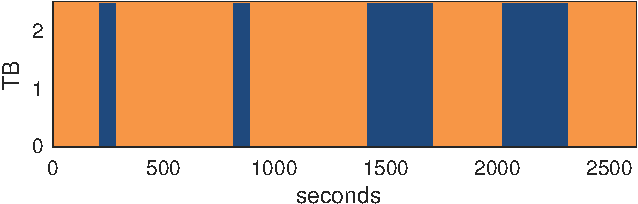
\includegraphics[width=0.8\linewidth]{fig/b1_mov_Optimum_BB}\label{fig:motiv-optimal}}	
%	\caption{Need for bounded priority and long-term fairness in a shared multi-resource cluster.
%    Although we only focus on memory allocations here, similar observations hold for other resources.}%In DRF, it is unfair for the first two jobs to slow down their progress although they require very small resources. From 0 to 1400 seconds, Strict speeds up the delay-sensitive jobs from \burstq but it later makes \batchq starving of resources because of the large jobs. \todo{change \burstq and \batchq to \burstq and \batchq}}
%	\label{fig:motiv_ex}
%\end{figure}

Consider the example in Figure~\ref{fig:motiv_ex} again. Recall that SP and DRF are two extreme cases in trading off performance and fairness: SP provides the best performance (for {\burstq}s) with no fairness consideration (for {\batchq}s); DRF ensures the best isolation (for {\batchq}s) with poor performance (of {\burstq}s). 
However, it is still possible for {\burstq}s and {\batchq}s to share the cluster by thoughtful co-scheduling over time.

The ideal allocation is depicted in Figure~\ref{fig:motiv-optimal}. 
The key idea is ``bounded'' priority for {\burstq}s as we discuss in the previous section. 
In particular, before 1,400 seconds, \burstq's bursts are small, so it gets higher priority, which is similar to SP. 
After \burstq increases its demand, only a fraction of its demand can be satisfied with the entire system's resources. Then it has to give resources back to \batchq to ensure the long-term fairness.

%in IQs unless we set very high weights to IQs. Even in this case, there are at least two problems: (a) BQ starvation, (b) still no performance guarantee with multiple IQs because giving them all high weights does not work.

%DRF/HUG: similar to FS as only focusing on instantaneous allocation.

%Strict priority (SP): BQ starvations
%
%\zhenhua{We should discuss other important schedulers. Mosharaf, could you please add some?}
%
%Figure: DRF/SP/DRFw/\name with small interactive queue: SP $>$ DRFw $>>$ DRF (\name performs similar to SP, better than DRFw, and much better than DRF)
%
%Figure: DRF/SP/DRFw/\name with small interactive queue: DRF $>>$ DRFw $>$ SP (\name performs similar to DRF, better than DRFw, and much better than SP)




%\emph{Example Setup} 
%
%\begin{itemize}
%\item Framework: Tez atop YARN.
%\item Assumption: All the jobs are memory bound jobs so that it is equivalent to single resource allocation.
%\item cluster: 40 nodes. each node has 64 GB RAM.
%\item \burstq submits delay-sensitive jobs. \burstq submits 4 Map Reduce jobs every 600 secs. A Map task <14GB, 1 cpu> resource takes 25 secs and a Reduce task <20GB, 1 cpu> takes 2 secs.
%	\begin{itemize}
%	\item 2 first jobs have 480 Map tasks and 80 Reduce tasks. 
%	\item The 3rd and 4nd jobs have 1920 Map tasks and 320 Reduce tasks. 
%	\end{itemize} 
%\item \batchq submits the jobs generated from BigBench workload. The \batchq's jobs are queued up at the beginning.
%\end{itemize}

%In Figure \ref{fig:mov_example}, Strict allows \burstq to speeds up his jobs to as soon as possible. However, Strict hurts \batchq a lot when the delay-sensitive jobs are too large (from 1000).





%\subsection{Just to organize our own thoughts}


\subsection{Desired Properties}
\label{sec:desire}

% \begin{figure}
% \centering
% 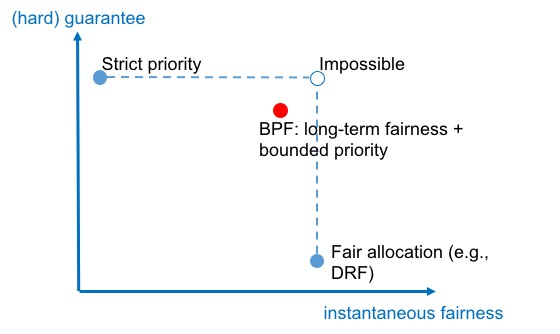
\includegraphics[scale=0.35]{fig/tradeoff}
% \caption{Design space -- \name provides {\burstq}s with bounded priority and maintains long-term fairness. \todo{I think we achieve fairness not bounded fairness.}}
% \label{fig:tradeoff}
% \end{figure}

We restrict our attention in this paper to the following, important properties: burst guarantee for {\burstq}s, long-term fairness for {\batchq}s, strategyproofness, and Pareto efficiency to improve cluster utilization.

\textbf{Burst guarantee (BG)} provides performance guarantee for {\burstq}s by allocating guaranteed amount of resources during their bursts. 
In particular, an {\burstq} requests its minimum required resources for its bursts to satisfy its service level agreements, e.g., percentiles of response time. 
%\xiao{Another things is that, I feel burst guarantee is promised by our admission control procedure, while other policies do not have such step. It's kind of unfair to compare to others using this property.}

%the key to provide service for latency-sensitive jobs, especially in latency-sensitive interactive analytics and online stream processing systems. In BPF, we provide as many LQ queues with burst guarantee as possible, given the long-term fairness ensured for both LQ and TQ queues.

\textbf{Long-term fairness (LF)} provides every queue in the system the same amount of resources over a (long) period, e.g., 10 minutes.
Overall, it ensures that {\batchq}s progress no slower than any {\burstq} in the long run. LF implies sharing incentive, which requires that each queue should be better off sharing the cluster, than exclusively using its own static share of the cluster. 
If there are $n$ queues, each queue cannot exceed $\frac{1}{n}$ of all resources under a static sharing.\footnote{For simplicity of presentation, we consider queues with the same weights, which can be easily extended to queues with different weights.}

\textbf{Strategyproofness (SPF)} ensures that queues cannot benefit by lying about their resource demands. 
This provides incentive compatibility, as a queue cannot improve its allocation by lying. 

\textbf{Pareto efficiency (PE)} is about the optimal utilization of the system. 
A resource allocation is Pareto efficient if it is impossible to increase the allocation/utility of a queue without hurting at least another queue. %This property is important as it leads to maximizing system utilization subject to satisfying the other properties.



\subsection{Analysis of Existing Policies}
\label{sec:property-analysis}


\begin{table}[!t]
	\small
	\centering
	\begin{tabular}{ |c||c|c|c||c| } 
		\hline
		Property  & SP  & DRF  & M-BVT  & BPF \\   [0.5ex] 
		\hline\hline
		Burst Guarantee (BG)    &  \checkmark* &$\times$ & \checkmark*  &\checkmark \\ 
		Long-Term Fairness (LF) & $\times$ & \checkmark &\checkmark &  \checkmark \\
		%Sharing Incentive (SI)  & $\times$ &\checkmark &\checkmark & \checkmark \\ 
		Strategyproofness (SPF)  & $\times$ & \checkmark& $\times$ & \checkmark\\
		Pareto Efficiency (PE)  & \checkmark & \checkmark &\checkmark & \checkmark \\
		\hline \hline 
		Single Resource Fairness & $\times$  & \checkmark & \checkmark & \checkmark \\
		Bottleneck Fairness & $\times$  & \checkmark & \checkmark & \checkmark \\
		Population Monotonicity & \checkmark  & \checkmark & \checkmark & \checkmark \\
		\hline
	\end{tabular}
	\caption{Properties of existing policies and {\name}. $\checkmark^*$ means that the property holds when there is only one \burstq.}
	%\todo{Define the asterisk for BG-SP combination here.}
	\label{tab-properties}
	\vspace{-0.1in}
\end{table}


%\todo{rewrite the following section}

\textbf{Strict Priority (SP): }
SP is employed to provide performance guarantee for {\burstq}s. As the name suggests, an SP scheduler always prioritize {\burstq}s. Therefore, when there is only one \burstq, SP provides the best possible performance guarantee. 
However, when there are more than one {\burstq}s, it is impossible to give all of them the highest priority. Meanwhile, {\batchq}s may not receive enough resources, which violates long-term fairness. As the {\burstq}s may request more resources than what they actually need, strategyproofness is not enforced, and therefore the system may waste some resources -- i.e., it is not Pareto efficient. 

%A danger with this type of service is that a queue can potentially starve out lower-priority traffic classes. 
%
%Obviously strict priority has burst guarantee for LQs and it is pareto-efficient. But for other properties it does not hold. For example, sharing is bad for those queues with lower-priority as they can be delayed for an infinite long time. And it is not a strategy-proofness as it can require all resources by claiming a very high priority level.   

\textbf{DRF:}  
DRF is an extension of max-min fairness to the multi-resource environment, where the dominant share is used to map the resource allocation (as a vector) to a scalar value. 
It provides instantaneous fairness, strategyproofness, and Pareto efficiency. %In particular, the strategyproofness property is straightforward in the single-resource environment but needs careful treatments in the multi-resource environment. 
However, because DRF is an instantaneous allocation policy without any memory, it cannot prioritize jobs with more urgent deadlines. In particular, no burst guarantee is provided. %Meanwhile, DRF is memoryless, it does not consider the time dimension, which is an important bridge between fairness and burstness. 
Even assigning queues different weights in DRF is homogeneous over time and cannot provide the burst guarantee needed. In addition, there is no admission control. Therefore, as the number of queues increases, no queue's performance can be guaranteed.

\textbf{M-BVT: }
BVT~~\cite{bvt} was designed as a scheduler for a mix of real-time and best-effort tasks. The idea is that for real-time tasks, BVT allows them to borrow some virtual time (and therefore resources) from the future and be prioritized for a period without increasing their long-term shares. 

To make it comparable, we extend it to M-BVT for a multi-resource environment.
Under the M-BVT policy, \burstq-$i$ is assigned a virtual time warp parameter $W_i$, which represents the urgency of the queue. Upon an arrival of its burst at $A_i$, an effective virtual time $E_i = A_i-W_i$ is calculated. This is used as the priority (smaller $E_i$ means higher priority) for scheduling. When \burstq-$i$ has the only smallest $E_i$, it may use the whole system's resources and its $E_i$ increases at the rate of its progress calculated by DRF. Eventually, its $E_i$ is no longer the only smallest. Then resources are shared in a DRF-fashion among queues with the smallest virtual times.


%until other queues catch up with \burstq-$i$ or there is some change to the system, e.g., a completion or an arrival of the {\burstq}s. 

The M-BVT policy has some good properties. For instance, the DRF component ensures long-term fairness, and the BVT component strives for performance. Pareto efficiency follows from the work conservation of the policy. 

However, it does not provide general burst guarantees as any new arriving queue (with larger virtual time warp parameter) may occupy the resources of existing {\burstq}s or share resources with them, thus hurting their completion time. In addition, it is not strategyproof because queues can lie about their needs in order to get a larger virtual time warp. 


%DRFQ tries to generalize fair queuing of packets from different flows, where packet consume multiple resources. It is an expansion from DRF and broaden the concept of fairness from space to time dimension with the idea of balancing virtual time, which has some similarity as our contribution. 

%Although DRFQ is used in packet environment, with a bit modification we can also apply it to datacenter scenario. And it have all properties mentioned above except burst guarantee. To allow special treatment for latency-sensitive queues, we need an extra virtual time warp parameter $w$ in BVT paper. The function of $w$ is similar to priority level, but it does not change the long-term share of different queues. However, it's does not have burst guarantee as any new arriving queue with larger $w$ may occupy your resources or share resource with you, thus hurting the completion time. And it's not a strategy-proof as there is no way to prevent user from lying.




\textbf{Other policies} such as the CEEI~\cite{moulin2014cooperative} provide fewer desired properties. 
%\zhenhua{I commented the details of PDRF and CEEI for now}

%\textbf{Proportional Dominant Share Fairness (PDRF):}
%Proportional fairness is a compromise-based scheduling algorithm. It assign different weight to different queues while tries to maximize the total output. We can also apply dominant share here as the following: For TQ$i$, we assign her unit weight and for LQ$j$, we assign her weight $\frac{1}{t}$ where $t$ is the percentage of her ON period divided by her total periodic length.
%
%Then we can directly use DRF to maxmin the weighted dominant share of all queues. Obviously, PDRF is pareto-efficient and sharing incentive. But similar to CEEI, it is not a strategy-proof and does not provide any burst guarantee for LQs. 
%
%
%\textbf{Competitive Equilibrium from Equal Incomes (CEEI):}
%We can also apply the method to fairly divide resources is Competitive Equilibrium from Equal Incomes (CEEI) from microeconomic theory. 
%
%The CEEI allocation is given by the Nash bargaining solution. The Nash bargaining solution picks the feasible allocation that maximizes $\prod_i u_i(a_i)$ where $u_i(a_i)$ is the utility that user $i$ gets from her allocation $a_i$. To support latency-sensitive queues, we can modify the utility function of these LQ queues. For example, we can set the utility for TQ$i$ simply her dominant share $s_i$, the utility for LQ$j$ is $s_i^{t}$, where $t$ is the percentage of her ON period divided by her total periodic length. 
%It's easy to see that CEEI is sharing incentive and pareto-efficient. However, CEEI is not a strategy-proof as she can get more burst speed by claiming a shorter ON period; Also, CEEI does not have burst guarantee for LQ jobs as here no fixed amount of resources is guaranteed for LQ queues.    

\subsection{Summary of the Tradeoffs}

As listed in Table~\ref{tab-properties}, no prior policy can simultaneously provide all the desired properties of fairness/isolation for {\batchq}s while providing burst guarantees for all the {\burstq}s with strategyproofness. In particular, if strict priority is provided to an \burstq without any restriction for its best performance (e.g., SP), there is no isolation protection for {\batchq}s' performance. On the other hand, if the strictly instantaneous fairness is enforced (e.g., DRF), there is no room to prioritize short-term bursts. While the idea in M-BVT is reasonable, it is not strategyproof and cannot provide burst guarantee.

%The key observation that motivates this work is that one cannot simultaneously provide all the desired properties of fairness/isolation for {\batchq}s while providing burst guarantees for all the {\burstq}s (Table~\ref{tab-properties}). 
%In particular, SP provides the best performance (the lowest completion time) to {\burstq}s without any isolation protection for {\batchq}s' performance. 
%DRF provides ideal instantaneous fairness without burst guarantees for {\burstq}s.
%BVT -- even with its multi-resource extension with DRF -- is not strategyproof.
% It is impossible to obtain the best performance and instantaneous fairness at the same time because instantaneous fairness cannot accommodate short-term burst of {\burstq}s.
% Therefore, long-term fairness is enforced instead to give room for the short-term burst requirement for {\burstq}s.
% On the other hand, the burst size of {\burstq}s cannot be too large compared to its long-term fair share.
% For instance, consider a link with capacity 100 MBps and shared by one {\burstq} and one {\batchq}. The {\burstq} has ON status every 10 seconds. If its demand during the ON status is no larger than 500MB (0.5*100MBps*10s), we can prioritize this {\burstq}.
% However, if its demand exceeds 500MB, we cannot give it high priority without hurting {\batchq}'s long-term fair share.

The key question of the paper is, therefore, how to allocate system resources in a near-optimal way; meaning, satisfying all the critical properties in Table~\ref{tab-properties}.

%So the approach should focus on how to dynamically adjust allocations according to the demand and performance metrics.
%
%\textcolor{red}{Key question: does \name solve the problem? If so, what additional challenges should we tackle?}
%
%
%{\burstq}s: high value, time sensitive, hard to accommodate with guarantee
%
%Even with the same utilization level, the system with more {\burstq}s is likely to generate higher profits. 
%However, this makes the resource management more challenging. 
%
%Figure~\ref{fig:mov_example} shows the example for only one {\burstq}, where there is no resource contention among {\burstq}s. 
%This makes the scheduling relatively easier: we just need to give the (only) {\burstq} bounded guarantee over time. 
%With more than one {\burstq}s, naive admission control would result in a suboptimal number of admitted {\burstq}s.
%
%Admission control example:
%
%Resource contention example: add another {\burstq} with arrival at 900 to Figure~\ref{fig:mov_example}. 
%Solution can be SRPT, which decreases JCT.



%\subsubsection*{Challenge: Increase {\burstq} Utilization}
%\label{sec:challenge}
%
%Another metric beyond the performance-isolation tradeoff is the system utilization. However, it is more complicated when {\burstq}s and {\batchq}s coexist. 
%Often, {\burstq}s have high value and are time sensitive. Therefore, they are hard to be accommodated with resource guarantees. On the other hand, it is relatively easy to fill the cluster with (possible) low value, batch jobs.
%In other words, system utilization is no longer the sole metric and the composition of it needs to be examined. 
%
%In this spirit, we call the utilization of {\burstq}s with resource guarantees {\burstq} utilization, which is the third performance metric that operators are likely to be interested in.


%Techniques such as packing can help further increase ``good'' utilization. 
%Our current work is based on admission in an FCFS manner.

% We assume {\burstq}s submit their highest possible demand across bursts.
%\subsection{Challenge: uncertainties in an {\burstq}'s demand}
%
%If an {\burstq} knows the distribution, she can run a stochastic optimization to decide the parameters used in her request. \zhenhua{Do we have any data to support this?}
%
%If an {\burstq} has no knowledge or the distribution varies dramatically over time (such as Figure~\ref{fig:mov_example}), she needs to submit multiple requests over time by solving a (challenging) online problem.

% \subsection{Connections to networking}
% \label{sec:networking}
%
% \todo{add something or remove this subsection}
